%!TEX root = ../username.tex
\chapter{Background} \label{bg}

This section contains the background information necessary to understand the project.

\section[Markov Chains]{Markov Chains} \label{bg:markov}

\subsection{Definition} \label{bg:markov:definitions}

A Markov Chain is a type of discrete-time stochastic process, which means a Markov Chain is a sequence of random variables $\boldsymbol{X} = \{X_{n} | n \in I\}$ for some index set $I$.
Additionally, Markov Chains have the special property that they depend only on the immediate past state(s).
That is, for a first-order Markov Chain at time $n$, $$P(X_{n} = j \mid X_{0} = i_{0}, \ldots, X_{n - 1} = i_{i - 1}) = P(X_{n} = j \mid X_{n - 1} = i_{n - 1})$$ for a particular possible outcome $j$ of $X_{n}$ \cite{nierhaus_algorithmic_2009}.

This idea can also extend to higher-order Markov Chains.
A higher-order Markov process considers more than the single most recent state to determine the next state.
An $n$th order Markov Chain uses the previous $n$ states as the input to find the next state.

\subsection{Representations} \label{bg:markov:representations}

We can think of a Markov Chain as a directed graph, where each state is a node, each edge is a transition between states, and the probabilities of transitioning between states are represented by the edge weights.
See Figure \ref{fig:markovGraph} for a visual representation of this idea.

\begin{figure}[h]
	\centering
	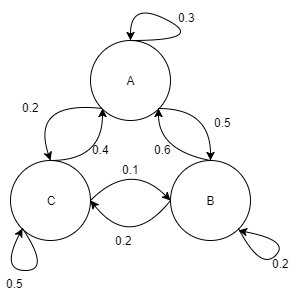
\includegraphics[]{figures/markovGraph.png} % TODO: Make a better diagram
	\caption{A Markov Chain represented as a graph.}
	\label{fig:markovGraph}
\end{figure}

When implementing a Markov Chain, however, it is perhaps easier to represent a is as an $(n + 1)$ dimensional array, where $n$ is the order of the Markov Chain.
See Figure \ref{fig:markovMatrix} for an example of the same Markov Chain as in Figure \ref{fig:markovGraph} in matrix form.

\begin{figure}[h]
	\centering
	\begin{tabular}{c | c c c}
		& $A_{1}$ & $B_{1}$ & $C_{1}$\\
		\hline
		$A_{0}$ & $0.3$ & $0.5$ & $0.2$\\
		$B_{0}$ & $0.6$ & $0.2$ & $0.2$\\
		$C_{0}$ & $0.4$ & $0.1$ & $0.5$
	\end{tabular}
	\caption{A Markov Chain represented as a transition matrix.}
	\label{fig:markovMatrix}
\end{figure}

\subsection{Limitations} \label{bg:markov:limitations}

A major limitation of Markov Chains is their inability to generate truly novel output.
In order for some state to appear, a transition to that state from the previous state must appear in the source.
Additionally, lower-order chains may produce nonsensical output, while a chain of sufficiently high order will exactly copy the source.
Another limitation is that the process may get stuck in a local loop.
This may happen when the chain proceeds to a state which only transitions to itself, or transitions to a set of states that only transition to each other.
